\documentclass[11pt,a4paper]{ctexart}
\usepackage[margin=1.9cm]{geometry}
\usepackage{amsmath,amssymb,bm}
\usepackage{booktabs,graphicx,xcolor,hyperref}
\hypersetup{colorlinks=true,linkcolor=blue,urlcolor=blue}
\setlength{\parindent}{2em}
\setlength{\parskip}{0.25em}
\makeatletter
\setlength{\@fptop}{0pt}
\makeatother
\title{IMU--UWB InEKF：原作者实现与改进版的公平算法对比}
\author{基于共同事件计划、预热和交替顺序的完整数据回放}
\date{2026年7月24日}

\begin{document}
\maketitle

\section{比较对象与计时边界}

原作者备份固定在提交
\texttt{f3b664e0e8c86b62c6ed2ea2a112261810228e1c}，其
\texttt{inekf.py} 以只读方式导入，没有修改。原始入口同时运行 InEKF、ESKF、
全数组时间戳扫描和交互绘图，不能与当前单滤波器入口直接比较。因此，本测试令
两套 InEKF 共享一个预计算事件计划，并仅计时滤波回放。

完整 const1 每轮对两边均调用
\[
N_{\mathrm{pred}}=142220,\qquad N_{\mathrm{UWB}}=67205.
\]
改进版还保留 11 次初始静止更新。数据读取、对象构造、历史记录、指标和绘图
全部在正式计时之外。数值库固定单线程，先分别预热 30\,s，再按
$AB/BA/AB/BA/AB/BA$ 完成六组配对。

\section{原论文形式与低开销实现}

原作者传播每个 IMU 步计算通用矩阵指数
\begin{equation}
 \Phi_{\mathrm{author}}=\exp(A\Delta t),
\end{equation}
并通过稠密块矩阵构造过程噪声。当前冻结误差矩阵满足 $A^4=0$，故改进版严格等价地
使用终止多项式
\begin{equation}
 \boxed{\Phi_{\mathrm{proposed}}
 =I+A\Delta t+\frac{1}{2}A^2\Delta t^2
 +\frac{1}{6}A^3\Delta t^3.}
\end{equation}
这不是截断近似。

令 $M=\Phi\operatorname{Ad}_{\hat X,\hat b}$，$d$ 为过程噪声对角向量，
则不再构造稠密对角阵：
\begin{equation}
 Q_d=M\operatorname{diag}(d)M^\mathsf{T}
 =\left(M\odot\bm{1}d^\mathsf{T}\right)M^\mathsf{T}.
\end{equation}
对一维 TDoA，令 $u=PH^\mathsf{T}$、$S=Hu+R$，标量更新写为
\begin{equation}
 \delta x=\frac{u r}{S},\qquad
 \boxed{P^+=P^--\frac{uu^\mathsf{T}}{S}},
\end{equation}
与 Joseph 形式在精确算术下等价。现有
$H_{\mathrm{left}}\operatorname{Ad}_{X^{-1}}$ 直接展开，常角速度 IMU
传播使用共享三角函数的 $\Gamma_1/\Gamma_2$ 闭式积分。这些结构化变化保留
15 维不变卡尔曼滤波主题，没有通过降维、降频或删掉 UWB 调用获得速度。

\section{完整 const1 计时}

\begin{table}[h]
\centering
\caption{六轮预热后正式回放，单位为秒。}
\begin{tabular}{ccccc}
\toprule
轮次 & 顺序 & 原作者 & proposed & 配对加速\\
\midrule
1 & 作者$\to$改进 & 45.5002 & 18.7047 & 2.4326\\
2 & 改进$\to$作者 & 44.6035 & 18.7208 & 2.3826\\
3 & 作者$\to$改进 & 44.4922 & 18.5902 & 2.3933\\
4 & 改进$\to$作者 & 44.7412 & 18.6291 & 2.4017\\
5 & 作者$\to$改进 & 44.5381 & 18.6217 & 2.3917\\
6 & 改进$\to$作者 & 44.5172 & 18.6012 & 2.3932\\
\midrule
中位数 & -- & 44.5708 & 18.6254 & \textbf{2.3933}\\
\bottomrule
\end{tabular}
\end{table}

预测与更新内核中位数为 44.1506\,s 和 18.2856\,s，配对中位加速
2.4147 倍；统一回放耗时下降 58.21\%。原作者和改进版回放 MAD 分别仅
0.0661\,s 和 0.0297\,s，顺序反转没有改变结论。由此可知，40--60\,s 的
旧印象与原作者 InEKF 核心量级吻合，而当前十几秒回放并非漏掉数据。

\section{精度与不可隐藏的代价}

\begin{table}[h]
\centering
\caption{额外完整精度回放；该回放不进入正式耗时统计。}
\begin{tabular}{lrrr}
\toprule
指标 & 原作者 & proposed & 相对变化\\
\midrule
位置 RMSE / m & 0.108003 & 0.097396 & $-9.82\%$\\
速度 RMSE / (m/s) & 0.060901 & 0.052396 & $-13.97\%$\\
姿态测地 RMSE / rad & 0.063826 & 0.081477 & $+27.65\%$\\
yaw RMSE / rad & 0.062300 & 0.081096 & $+30.17\%$\\
UWB 拒绝数 & 0/67205 & 0/67205 & 相同\\
\bottomrule
\end{tabular}
\end{table}

改进版的 2\,rad 全圆未知 yaw 先验用于避免大初始航向误差时的过度自信；
const1 的真实初始 yaw 恰好接近 $0^\circ$，因此该保守先验在本条数据产生约
24\,s 的初始瞬态，使全程姿态/yaw RMSE 变差。后半程改进版 yaw 误差通常更低。
因此本结果只能表述为“位置、速度和计算开销改善，付出初始 yaw 瞬态代价”，
不能宣称全部精度指标都提升。

\begin{figure}[p]
\centering
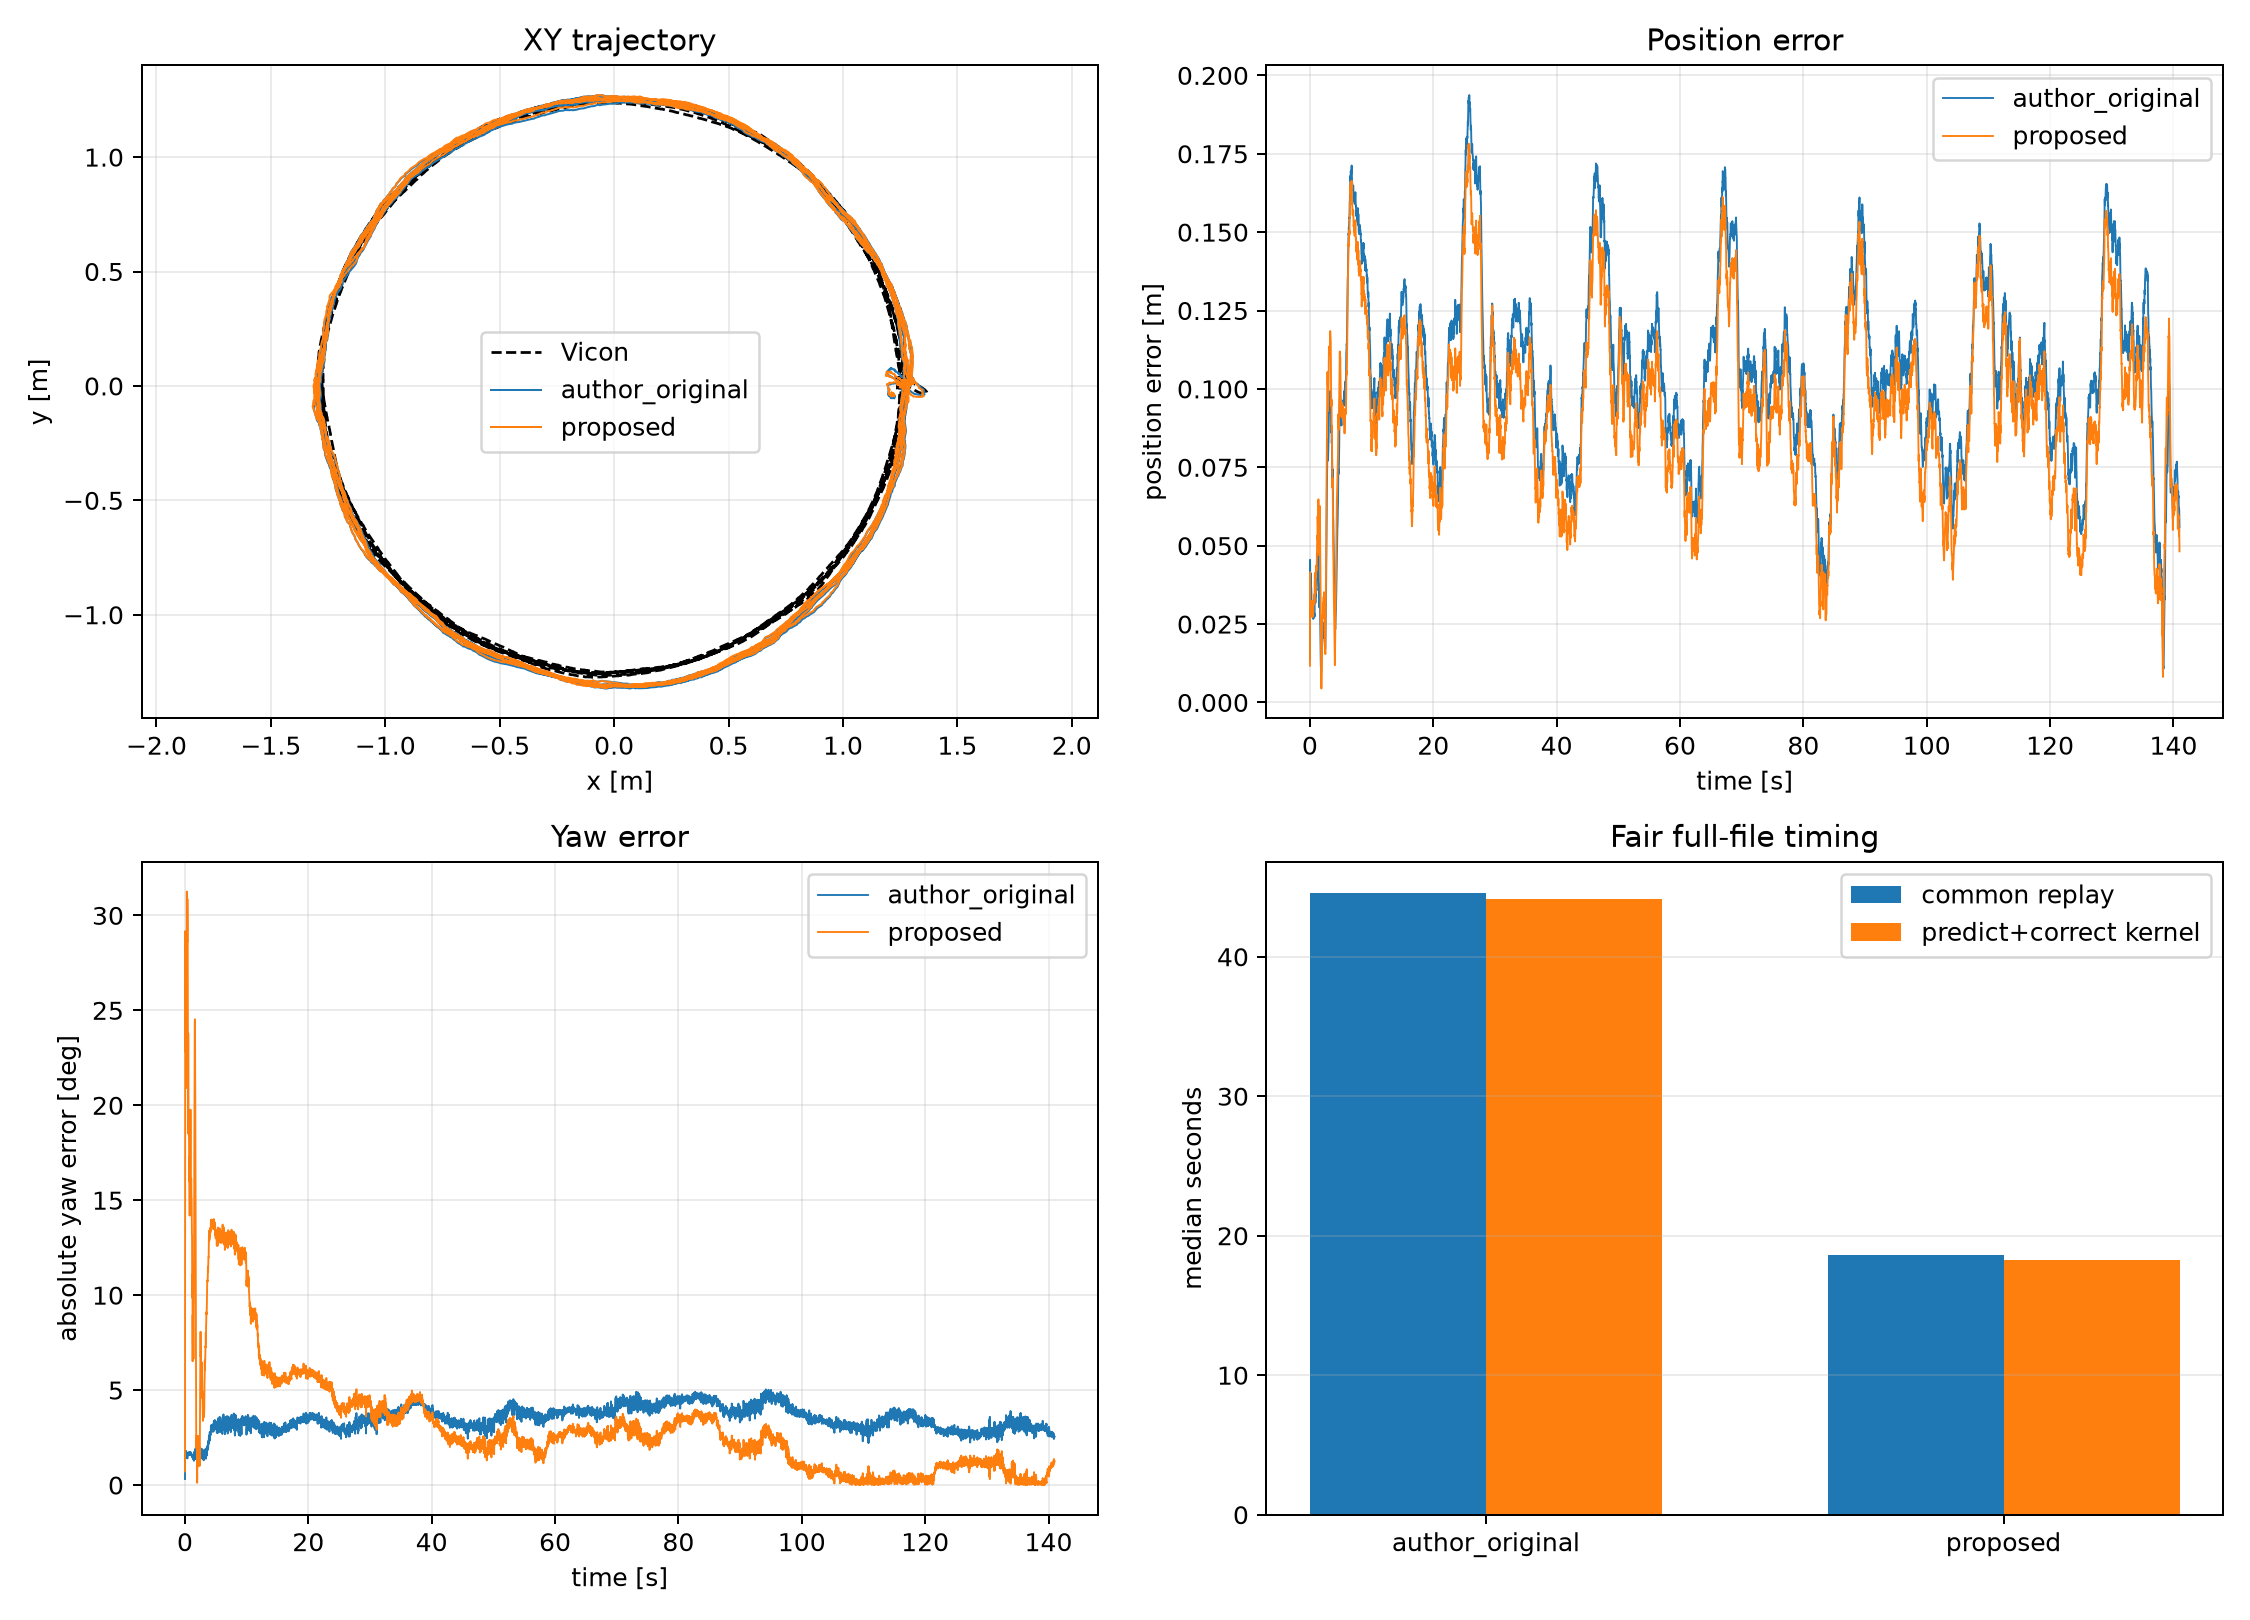
\includegraphics[width=\textwidth]
{../imu-uwb-inekf/results/fair_author_original_vs_proposed_const1_full/comparison.png}
\caption{共同调度下的轨迹、位置误差、yaw 误差与正式耗时中位数。两条轨迹连续，
无异常跳变或发散。}
\end{figure}

\section{结论与边界}

在本机 Windows、指定 Conda 环境、单线程和完整 const1 上，当前
\texttt{proposed} 相对原作者未修改 InEKF 的公平回放加速为
\textbf{2.3933 倍}。该值不含加载、构造、绘图或另一套 ESKF，也不等同于
嵌入式 WCET。更换机器、数值库或数据集后应以同一预热和交替脚本复测。

\end{document}
